\subsection{Graph Database} \label{subsec:graph_database}
% Checked - all edges are created with 'match' statement
% todo check numbers of Protein Edges!! current number is only proteins directly on genes
% TODO Bezeichnung der IDs in Cypher Queries nochmal prüfen
% TODO check final version of the Cypher query for gene nodes with all attributes

% Intro
As we have created our base data models, our next objective~\ref{obj:graph_algorithm} is to create a graph database
that can be used to perform the PageRank algorithm as a graph algorithm.
With four huge datasets at our disposal, optimizing the generation of the database is crucial.
In this section, we describe the queries, called cypher queries, used to create and populate our graph database,
including information about creating indexes, constraints, relationships between nodes, and loading data into the database.\\


% PPI Network
To construct the \textbf{basic PPI network}, we need to create protein nodes and their interactions as edges.
To optimize query execution, we start with indexing the protein property $ID$.
Next we load the data (\ref{subsubsec:protein_nodes}~-~Protein nodes) as a list and then create the nodes in batches for efficient processing.
The graph database is populated with 104,235 protein nodes.

Since these nodes are used solely for connections between genes, no additional properties are required.
The cypher query for creating protein nodes is:

\begin{lstlisting}[language=Cypher, label={lst:protein_nodes}]
    CREATE (p:protein {id: 'Protein ID'})
\end{lstlisting}


We then create interaction edges by loading the saved data (\ref{subsubsec:protein_protein_edges}~-~Protein-protein edges)
as a list of protein tuples and searching for both protein nodes by their ID in the graph database.
The edges are created in batches for efficient processing, resulting in 11,247,242 interactions between protein nodes.

The cypher query for creating protein-protein edges is:

\begin{lstlisting}[language=Cypher, label={lst:protein_edges}]
    MATCH (s:protein{id:'left Protein ID'})
    MATCH (s:protein{id:'right Protein ID'})
    CREATE (s)-[:interaction]->(t)
\end{lstlisting}

We now have a complete PPI network in place.\\

% MATCH p=()-[r:interaction]->() RETURN p LIMIT 5
\begin{figure}[h]
    \centering
    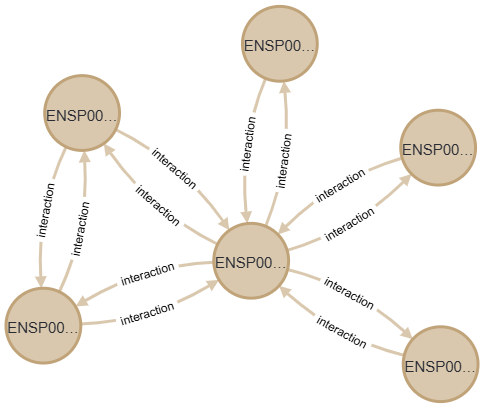
\includegraphics[width=0.35\textwidth]{figures/03_03_Basic_Network}
    \caption{Extract from the graph database setup showing example protein nodes and their interactions.}
    \label{fig:03_03_Basic_Network}
\end{figure}



%%%%%%%%%%%%%%%%%%%%%%%%%%%%%%%%%%%%%%%%%%%%%%%%%%%%%%%%%%%%%%%%%%%%%%%%%%%%%%%%%%%%%%%%%%%%%%%%%%%%%%%%%
% Extending the Network with Genes
Our actual focus is on the genes.
For constructing our \textbf{extended PPI network} with genes on the edges of the protein nodes, we need to connect them to the proteins.
To achieve this, we first create gene nodes with their associated attributes,
utilizing efficient data loading techniques to facilitate faster query execution.
Specifically, we implement an index on the gene property id to expedite querying,
load the data as a list, create nodes in batches to optimize processing,
and ultimately populate the graph database with 17,626 gene nodes.

The Cypher query employed for creating these gene nodes is:
\begin{lstlisting}[language=Cypher, label={lst:gene_nodes}]
    CREATE (p:gene {
            id: 'id',
            gene_name: 'gene_name',
            norm_healthy_tpm: 'norm_healthy_tpm',
            norm_cancerous_tpm: 'norm_cancerous_tpm',
            delta_tpm: 'delta_tpm',
            delta_type: 'delta_type',
            delta_tpm_relevant: 'delta_tpm_relevant'})
\end{lstlisting}

The genes in our network will be characterized by several properties:
$gene\_name$, $norm\_healthy\_tpm$, $norm\_cancerous\_tpm$, $delta\_tpm$, and $delta\_type$.


Among these, the calculation of $delta\_tpm\_relevant$ stands out as a pivotal factor in our analysis.
Although other attributes may be less relevant to our current investigation, they retain potential value for future tasks.

To model relationships between genes and proteins,
we establish connections between these nodes by loading gene-protein interaction data as a list of tuples.
This involves matching both gene and protein nodes based on their respective Ids,
and creating edges in batches to optimize processing efficiency.
The result is a comprehensive network of 101,731 connections between gene and protein nodes

The Cypher query for creating gene-protein connection edges is:
\begin{lstlisting}[language=Cypher, label={lst:gene_protein_edges}]
    MATCH (s:protein{id:'Protein ID'})
    MATCH (s:gene{id:'Gene ID'})
    CREATE (s)-[:connection]-(t)
\end{lstlisting}

% TODO Alternativ Verlinkung zu oben
\begin{figure}[h]
    \centering
    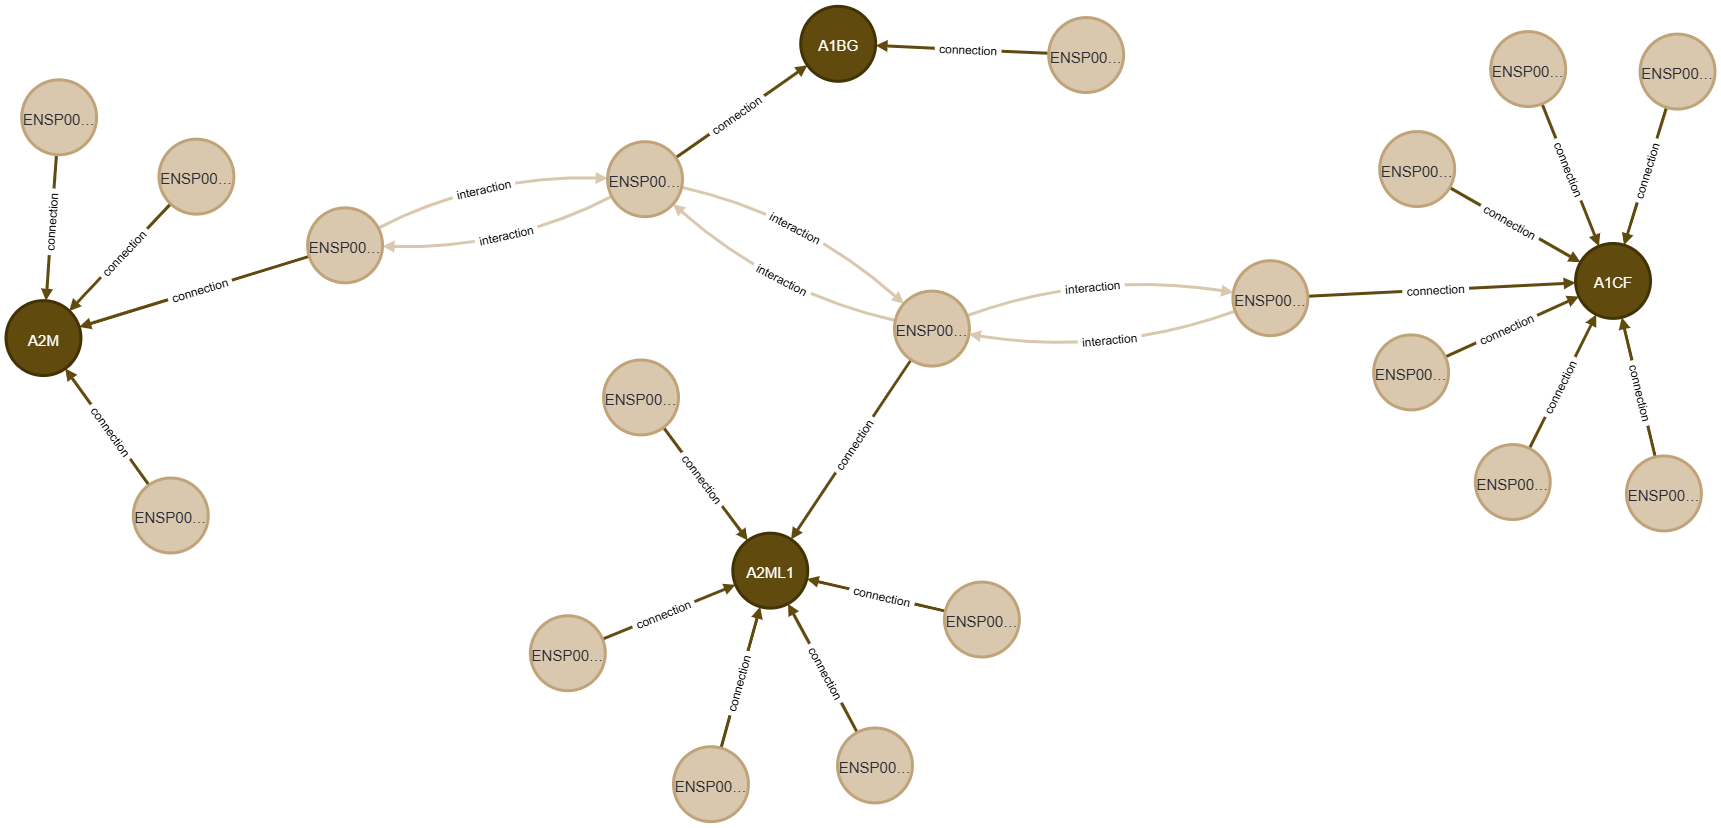
\includegraphics[width=1\textwidth]{figures/03_02_Network_2}
    \caption{Extract from the graph database setup ...}
    \label{fig:03_02_Network_2}
\end{figure}

Through the execution of these Cypher queries,
we are able to populate our graph database with the necessary nodes and edges to perform the PageRank algorithm.\\